\documentclass[a4paper,12pt]{article}

%%% Работа с русским языком
\usepackage{cmap}					% поиск в PDF
\usepackage{mathtext} 				% русские буквы в формулах
\usepackage[T2A]{fontenc}			% кодировка
\usepackage[utf8]{inputenc}			% кодировка исходного текста
\usepackage[english,russian]{babel}	% локализация и переносы
\usepackage{comment}


%%% Дополнительная работа с математикой
\usepackage{amsfonts,amssymb,amsthm,mathtools} % AMS
\usepackage{amsmath}
\usepackage{icomma} % "Умная" запятая: $0,2$ --- число, $0, 2$ --- перечисление

%% Номера формул
%\mathtoolsset{showonlyrefs=true} % Показывать номера только у тех формул, на которые есть \eqref{} в тексте.

%% Шрифты
\usepackage{euscript}	 % Шрифт Евклид
\usepackage{mathrsfs} % Красивый матшрифт

\usepackage{extsizes} % Возможность сделать 14-й шрифт
\usepackage{geometry} % Простой способ задавать поля
\geometry{top=25mm}
\geometry{bottom=35mm}
\geometry{left=20mm}
\geometry{right=20mm}

\usepackage{chngcntr}
\usepackage{hyperref}

\usepackage{setspace} % Интерлиньяж
%\onehalfspacing % Интерлиньяж 1.5
%\doublespacing % Интерлиньяж 2
%\singlespacing % Интерлиньяж 1

\usepackage{lastpage} % Узнать, сколько всего страниц в документе.
\usepackage{soulutf8} % Модификаторы начертания

\counterwithin*{equation}{section}
\counterwithin*{equation}{subsection}



%% Свои команды
\DeclareMathOperator{\sgn}{\mathop{sgn}}

%% Перенос знаков в формулах (по Львовскому)
\newcommand*{\hm}[1]{#1\nobreak\discretionary{}
{\hbox{$\mathsurround=0pt #1$}}{}}

%%% Работа с картинками
\usepackage{graphicx}  % Для вставки рисунков
\graphicspath{{images/}{images2/}}  % папки с картинками
\setlength\fboxsep{3pt} % Отступ рамки \fbox{} от рисунка
\setlength\fboxrule{1pt} % Толщина линий рамки \fbox{}
\usepackage{wrapfig} % Обтекание рисунков и таблиц текстом

%%% Работа с таблицами
\usepackage{array,tabularx,tabulary,booktabs} % Дополнительная работа с таблицами
\usepackage{longtable}  % Длинные таблицы
\usepackage{multirow} % Слияние строк в таблице
\usepackage{graphicx}
\usepackage{fancyhdr}
\usepackage{hyperref}
\usepackage{booktabs}

\newcommand{\lt}{\left}
\newcommand{\rt}{\right}
\newcommand{\al}{\alpha}

\pagestyle{fancy}
\fancyhf{}
\pagestyle{plain} % нумерация вкл.

\rhead{\today}
\lhead{Соколов Игорь, группа 573}

%%% Заголовок
\author{Соколов Игорь, группа 573}
\title{ДЗ 4 по Методам Оптимизации. \newline Сопряженные множества. Двойственные конусы. Многогранники. Лемма Фаркаша}
\date{\today}

\begin{document} % конец преамбулы, начало документа

\maketitle

\section{}

Найти и изобразить на плоскости множество, сопряженное к многогранному конусу: $$ S = \mathbf{conv} \left\{ (-4,-1), (-2,-1), (-2,1)\right\} + \mathbf{cone} \left\{ (1,0), (2,1)\right\} $$

\vspace{\baselineskip}

\textbf{Решение:}

Приведем теорему из семинара:

Пусть $x_1,\ldots,x_m \in\mathbb{R}^n$. Сопряженным к многогранному множеству:
 $$ \textbf{S} = \mathbf{conv}\{x_1, \ldots, x_k\} + \mathbf{cone}\{x_{k+1}, \ldots, x_m \}$$
 
является полиэдр (многогранник):
\[\textbf{S} = \left\{p \in \mathbb{R}^n \mid \langle{ p, x_i }\rangle \ge -1, i = \overline{1, k}; \langle{ p, x_i }\rangle \ge 0 , i =\overline{k+1, m} \right\} \]

Используя теорему:
\[\textbf{S*} = \{p \in \mathbb{R}^n \mid -4p_1 - p_2 \ge -1\textbf{,} - 2p_1 -p_2 \ge -1\textbf{,} -2p_1 + p_2 \ge -1 \textbf{,} p_1 \ge 0 \textbf{,} 2p_1 + p_2 \ge 0\}\]

Таким образом имеем систему:
\[
\left\{
\begin{aligned}
p_2 &\leq -4p_1 + 1  \\
p_2 &\leq -2p_1 + 1\\
p_2 &\ge 2p_1 - 1\\
p_1 &\ge 0  \\
p_2 &\ge -2p_1
\end{aligned}
\right.
\]

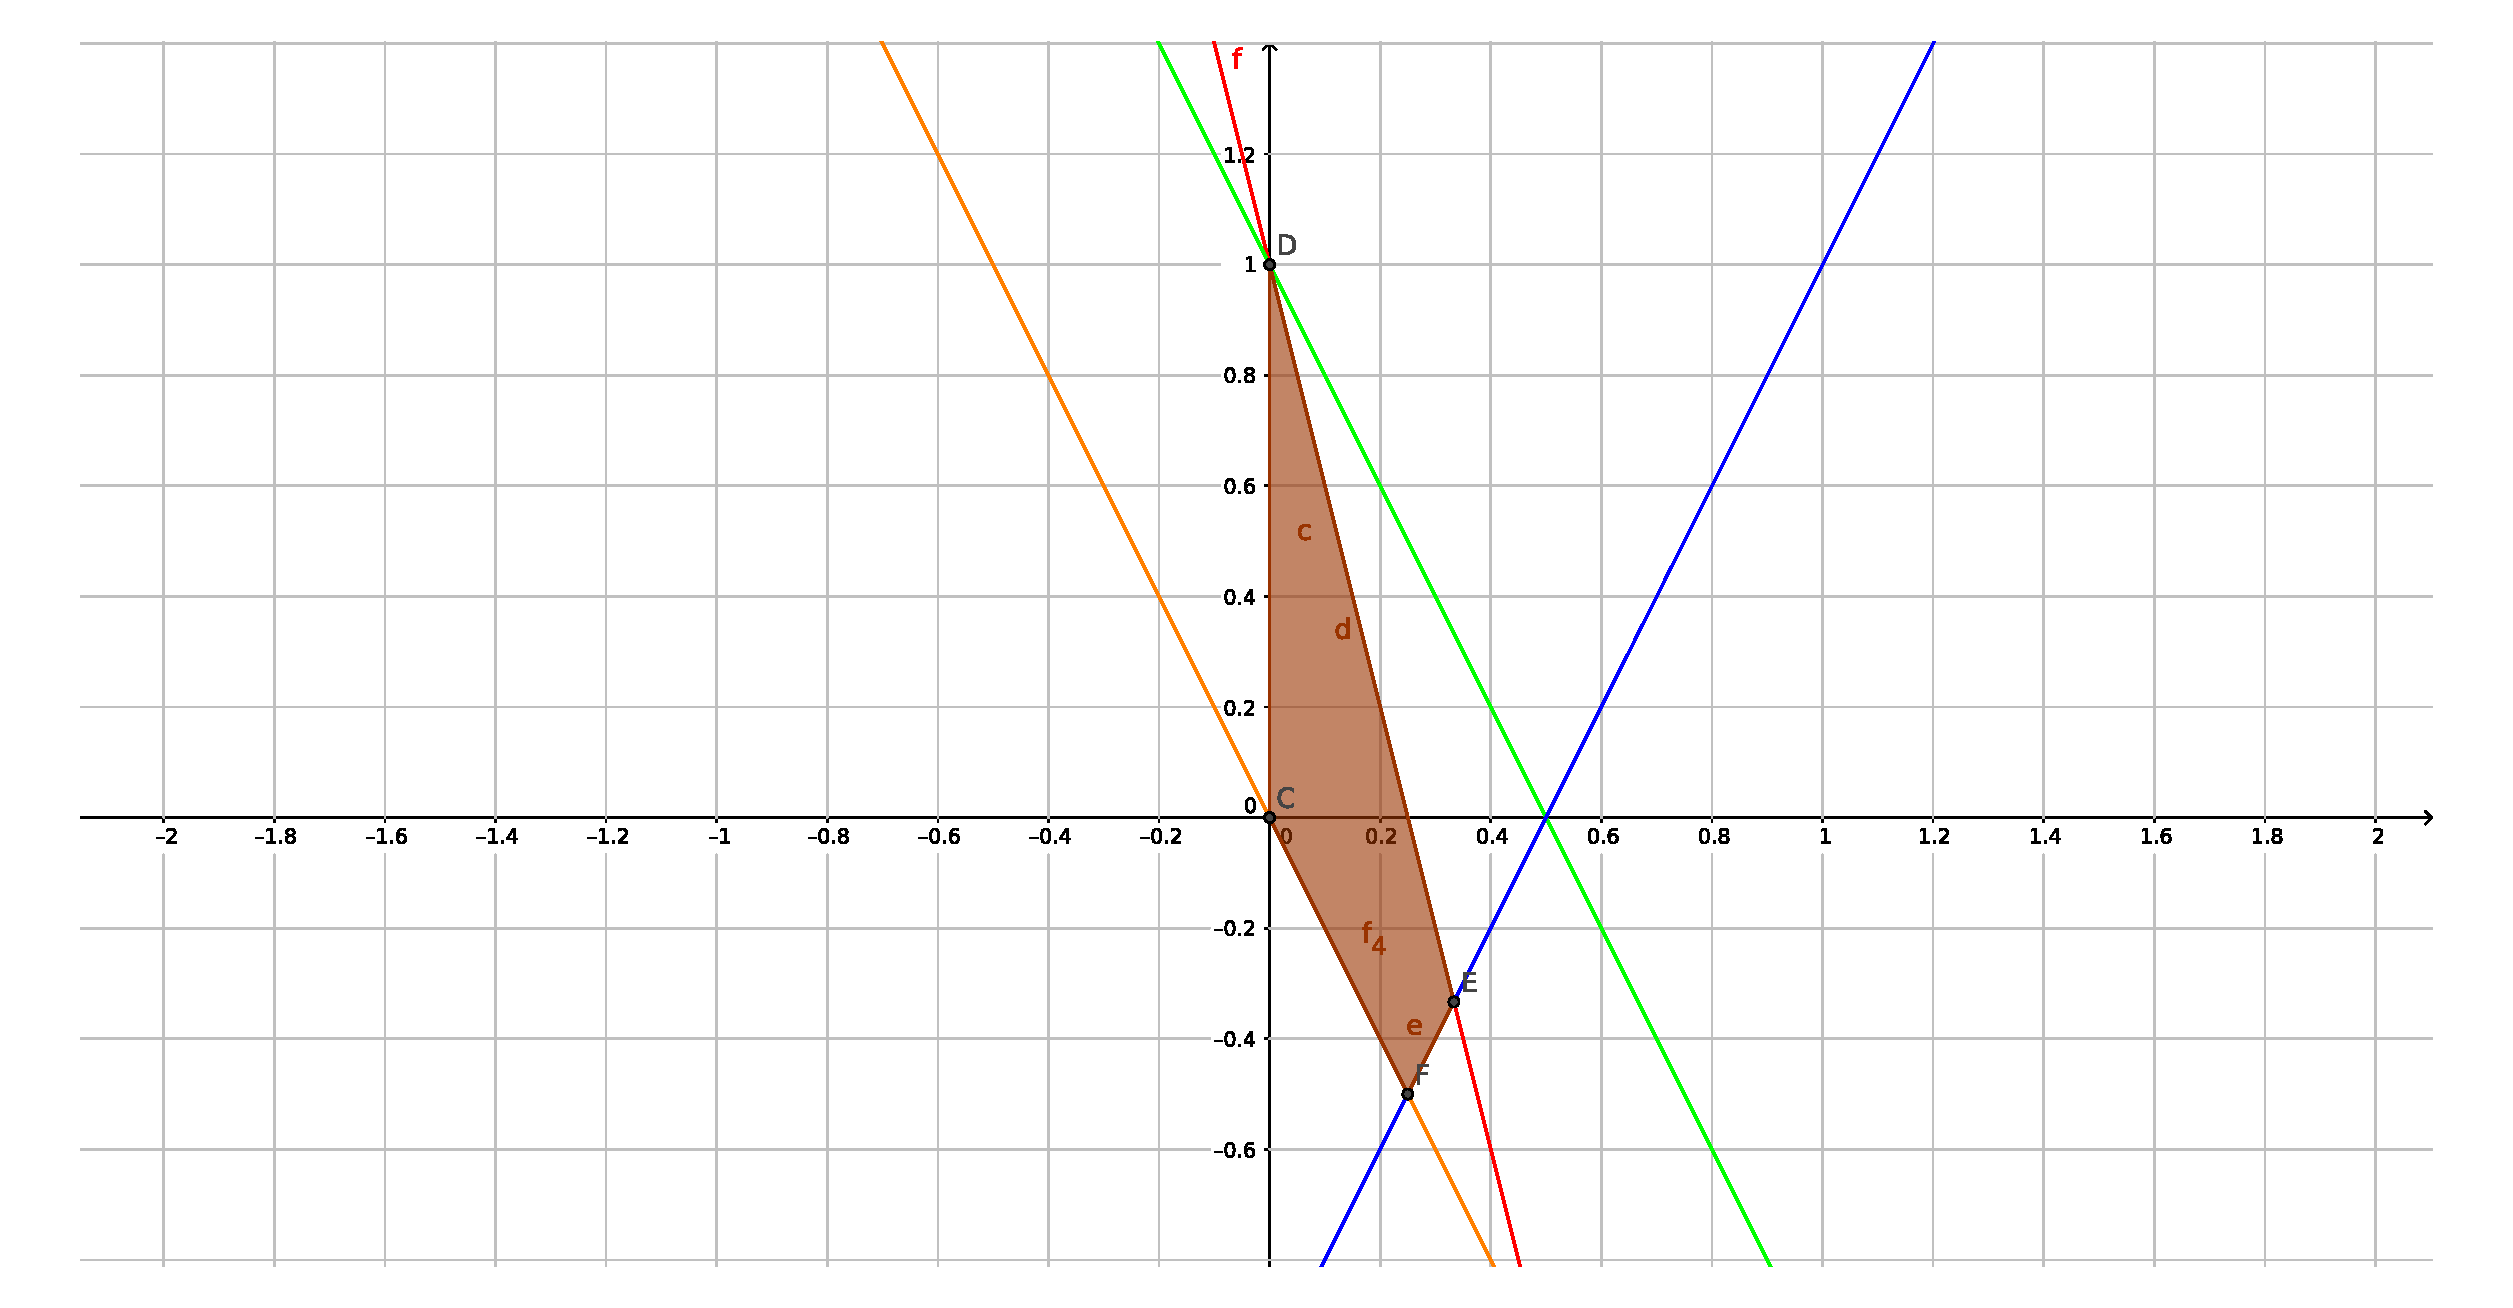
\includegraphics[width=\textwidth]{image_problem1.pdf}

\vspace{\baselineskip}

\section{}

Найти и изобразить на плоскости множество, сопряженное к полиэдру: $$S = \left\{ x \in \mathbb{R}^2 \mid -3x_1 + 2x_2 \le 7, x_1 + 5x_2 \le 9, x_1 - x_2 \le 3, -x_2 \le 1\right\}$$

\vspace{\baselineskip}

\textbf{Решение:}

\vspace{\baselineskip}


\textbf{Ответ:}

%3

\section{}

Доказать, что если понятие сопряженного множества к множеству $S$ вводить как: $$S^* = \{y \ \in \mathbb{R}^n \mid \langle y, x\rangle \le 1 \;\; \forall x \in S\}, $$ то единичный шар с центром в нуле - единственное самосопряженное множество в $\mathbb{R}^n$.

\vspace{\baselineskip}

\textbf{Решение:}

\vspace{\baselineskip}

\textbf{Ответ:}

%4
\section{}

Найти множество, сопряженное к эллипсоиду: $$ S = \left\{ x \in \mathbb{R}^n \mid \sum\limits_{i = 1}^n a_i^2 x_i^2 \le \varepsilon^2 \right\}$$

\vspace{\baselineskip}

\textbf{Решение:}

\vspace{\baselineskip}

\textbf{Ответ:} 




\end{document} % конец документа

